
\documentclass[a4paper, 11pt]{article}
\usepackage[czech]{babel}
\usepackage[utf8]{inputenc}
\usepackage[left=2cm,text={17cm, 24cm},top=2cm]{geometry}
\usepackage{graphicx}

\usepackage[hyphens]{url}
\usepackage[]{algorithm2e}
\usepackage[unicode, colorlinks, hypertexnames=false, citecolor=red]{hyperref}
\usepackage{xcolor}
\usepackage{algorithmic}

\title{ifj_doc}
\author{}
\date{December 2021}
\renewcommand{\baselinestretch}{1.5}

\begin{document}
%----Titulna Strana----%
\begin{titlepage}
\begin{center}
\huge


\includegraphics[scale=0.8]{vutfitlogo.png}\vspace{2cm}

\textsc{\LARGE VYSOKÉ UČENÍ TECHNICKÉ V BRNĚ}\\
\Large FAKULTA INFORMAČNÍCH TECHNOLOGIÍ\vspace{4cm}


\LARGE Projektová dokumentace\\
\Large {\bf Světelná tabule}\\
\Large IMP - Mikroprocesorové a vestavěné systémy \\
\vspace{7cm}
\end{center}
\begin{tabular}{l c c}
    \textbf {Tadeáš Kachyňa} & (xkachy00) \\
\end{tabular}
     \hfill  \today
\end{titlepage}
\section{Úvod}
Maticové displeje jsou běžnou součástí našich životů, jsou zejména vhodné pro stavbu textových a grafických panelů. Když se řekne pojem "běžící text na maticovém displeji", tak se mi nejrycheji vybaví jednořádkový panel s textem informující cestující běžně umístněný ve vozidlech hromadné dopravy. A~ něco podobného, ale v mnohem menším provedení si vyzkouším v rámci předmětu na Mikroprocesorové a vestavěné systémy na FIT VUT v Brně. Zadáním projektu byl návrh a implementace jednoduché světelné tabule s běžícím textem na výukové desce FitKit3, která obsahuje mikrokontrolér KCU Freescale KINETIS(MK60DN512VMD10), viz manuál \cite{k60_manual}. K této desce byl připojen přípravek matiscový displej. Vestavěná aplikace byla implementována v jazyce C v prostředí KDE (Kinetis Design Studio).

\section{Problematika}
Přípravek "maticový displej" se skládá z 2ks maticového LED displeje s typovým 
označením KWM-30881AGB. Každý tento displej se skládá z řádků a sloupců, kde v daném sloupci sdílejí LED diody společnou anodu. Pomocí řádkových vodičů můžeme následně rozsvěcovat a zhasínat jednotlivé pozice ve sloupci.

\begin{figure}[!htb]
    \centering
    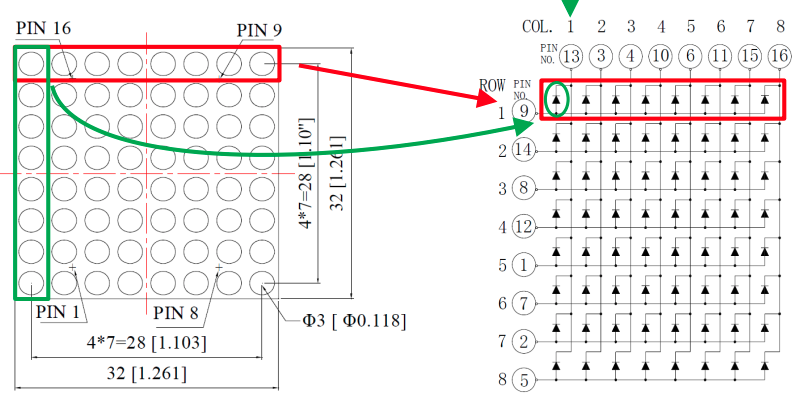
\includegraphics[scale=0.3]{maticovy_displej.png}
    \caption{Podrobné zobrazení řádkové a sloupcové problematiky uvnitř maticového displeje}
    \label{fig:my_label}
\end{figure}

\noindent Maticový displej zapojíme propojovacím konektorem P3 na vývody konektoru P1 umístněného na platformě FitKit3. Výsledný projekt má vykreslovat text běžící zprava doleva, používat multiplexing pro selekci sloupců a řádků, dovolit uživateli přepínat mezi předdefinovanými texty za pomocí tlačítek na platformě FitKit3 a využívat vestavěných modulů mikrokontroléru.

\newpage
\section{Popis řešení}
Implementace se nachází v souboru \texttt{main.c}.

\subsection{Inicializace MCU}
Ve funkci \texttt{MCUInit()} provedeme všechny potřebné kroky k správné konfiguraci mikrokontroléru než začneme zobrazovat text. To znamená správné nastavení pinů sloužících k ovládání sloupců a řádků pro GPIO funkcionalitu. Taktéž nastavíme a povolíme přerušení, které budeme vyvolávat při stisknutí tlačítek na platformě FitKit3 sloužicích k zobrazení různých textů na displeji a přerušení pro časovač LPTMR (Low Power Timer).

\subsection{Volba sloupců a řádků}
Selekce sloupců a řádů probíhá pomocí multiplexingu. Pro sloupce je tvořen dekodérem 4-16, kde za pomocí dekadické hodnoty 0-15, která bude násleně převedeno do binární podoby, zvolíme nultý až patnáctý sloupec. 

\noindent Řádky mapujeme hodnotami 0-255, která je poté převedena do binární ekvivalence a na základě jedniček a nul zvolíme, které řádky budou svítit a které zůstanou zhasuté.

\noindent Nesmíme ale opomenout, že v jeden okamžik může svítit pouze jeden sloupec. To vyřešíme nastavavením dostatečně vhodného zpoždění, kdy text bude problíkávat takovou rychlosti, že dokážeme zmást lidské oko, kterému se bude jevit, že sloupců svítí více.


\subsection{Tlačítka}
Na základě stisku tlačítek je vyvoláno přerušení, kde z hodnoty registru ISFR zjistíme, které tlačítko uživatel stisknul a zobrazíme na displeji příslušný text. Tlačítek je celkem 5.

\begin{figure}[!htb]
    \centering
    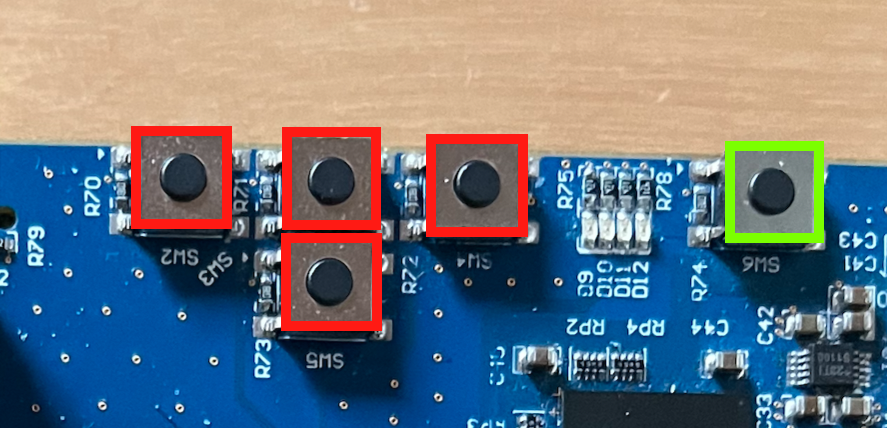
\includegraphics[scale=0.3]{buttons.png}
    \caption{Pohled na tlačítka na platformě FitKit3}
    \label{fig:my_label}
\end{figure}

\noindent Červenými tlačítky můžeme přepínat mezi předdefinovanými texty, modrým tlačítkem se vrátíme zpět k úvodnímu textu "Hello World" , který se nám zobrazí po spuštění programu.

\subsection{Posun textu}
K posouvání textu je využito vestavěného časovače LPTMR, který generuje přerušení v definovaném čase. Při prerušení dojde k posunu textu. Aby nám text tzv. "nepřetékal" z levé strany zpět na pravou, tak je ohraničen podmínkami, samotný algoritmus / funkce je popsána níže. \\
\hline \vspace{00.5cm}
\begin{algorithmic}
    \STATE \textbf{\#define} DISPLAY\_SIZE 16
    \FOR{(shift = 0; shift \textless \; text.length; shift++)}
    {\IF{(column \textgreater=  shift \textbf{and} column \textless \; DISPLAY\_SIZE + shift)}
        \STATE column\_select(column -- shift)
        \STATE rows\_selects(text[shift])
        \STATE delay()
      \ENDIF}    
\end{algorithmic}
\vspace{00.5cm}
\hline
\vspace{00.5cm}
\noindent Pokaždé když přijde k posunu, tak dojde ke kontrole pro každý sloupec, jestli se nachází v daném intervalu, který je dán jeho posunem a fyzickou velikostí maticového displeje. Pokud se v intervalu nachází, tak se rozsvítí daný sloupec a dané řádky a spustí se zpoždění.

\section{Závěr a zhodnocení}
Projekt byl úspěšně otestován na platformě FitKit3. Zdroje k projektu jsem hledal v přednáškách a~ cvičeních a~ v znalostech, které jsem si z nich odnesl. Z mého pohledu jsem naimplementoval vše, co bylo potřebné.
Ohledně zapojení komponent jsem čerpal z prezentace přiložené k zadání projektu \cite{prezentace}. K zprovoznění ostatních vestavěných komponent na platformě FitKit3 anebo informace ohledně registrů mi pomohly tyto materiály \cite{schemafitkit} \cite{k60_manual}.
Je mi radostí, že jsem si mohl vyzkoušet poprvé za studium práci s HW i doma na projektu, protože během doby covidové a~ ostatních hardware předmětů byla tato možnost značně limitována.

\section{Odkaz na demonstrační video}
Video je komentované, je vysvětlen základní princip vykreslování a demonstrace jednotlivých nadefinovaných textů.
Bohužel skrz (asi) rozdílnou frekvenci kamery a displeje se nepodařilo zachytit identický snímek zobrazovaného textu. \\ \vspace{00.5cm}

https://www.youtube.com/watch?v=JKwKPXEZOmQ

\section{Zdroje}
\bibliographystyle{czechiso}
\bibliography{documentation}
\end{document}
